\documentclass[10pt,journal]{IEEEtran}

% ── Preprint notice ──────────────────────────────────────────────────────────
% This is the author's preprint version. The paper has been submitted to
% IEEE Access and is currently under review.  This preprint does not use any
% IEEE-copyrighted material (class files, fonts, or formatting).
% Posting on arXiv is permitted under IEEE's preprint policy:
%   https://journals.ieeeauthorcenter.ieee.org/become-an-ieee-journal-author/
%   publishing-ethics/guidelines-and-policies/post-publication-policies/
% ─────────────────────────────────────────────────────────────────────────────

\usepackage{cite}
\usepackage{amsmath,amssymb,amsfonts}
\usepackage{algorithmic}
\usepackage{graphicx}
\usepackage{textcomp}
\usepackage{booktabs}
\usepackage{algorithm}
\usepackage{multirow}
\usepackage{url}

\begin{document}

\title{Comparative Analysis of 3D Convolutional and 2.5D Slice-Conditioned
U-Net Architectures for MRI Super-Resolution via Elucidated Diffusion Models}

\author{Hendrik Chiche, Ludovic Corcos, and Logan Rouge%
\thanks{Hendrik Chiche, Ludovic Corcos, and Logan Rouge are in collaboration with GENCI (Grand \'{E}quipement National de Calcul Intensif), France (e-mail: hendrik\_chiche@berkeley.edu; ludovic.corcos@etu.uca.fr; logan.rouge@etu.uca.fr). This work was supported in part by GENCI for access to high-performance computing resources.}%
}

\begin{abstract}
Magnetic resonance imaging (MRI) super-resolution (SR) methods that
computationally enhance low-resolution acquisitions to approximate
high-resolution quality offer a compelling alternative to expensive
high-field scanners.
In this work we investigate an elucidated diffusion model (EDM) framework
for brain MRI SR and compare two U-Net backbone architectures:
(i)~a full 3D convolutional U-Net that processes volumetric patches
with 3D convolutions and multi-head self-attention, and
(ii)~a 2.5D slice-conditioned U-Net that super-resolves each slice
independently while conditioning on an adjacent slice for inter-slice
context.  Both models employ continuous-sigma noise conditioning following
Karras et al.\ and are trained on the NKI cohort of the FOMO60K dataset.
On a held-out test set of 5~subjects (6~volumes, 993~slices), the 3D model achieves
\textbf{37.75\,dB PSNR}, \textbf{0.997 SSIM}, and \textbf{0.020 LPIPS},
improving on the off-the-shelf pretrained EDSR baseline
(35.57\,dB / 0.024 LPIPS) and the 2.5D variant (35.82\,dB) across all
three metrics under the same test data and degradation pipeline.
\end{abstract}

\begin{IEEEkeywords}
Brain MRI, convolutional neural network, denoising diffusion model,
elucidated diffusion model, image super-resolution, 3D U-Net.
\end{IEEEkeywords}

\maketitle

\begin{center}
\begin{minipage}{0.98\linewidth}
\footnotesize
\raggedright
\textit{Preprint notice:} This is a preprint of a paper submitted to
\textit{IEEE Access} and currently under peer review. The content is
identical to the submitted manuscript. This preprint is made available
under IEEE's author-posting policy.\\[2pt]
Source code: \url{https://github.com/Magic-Solutions/MRI-Super-Resolution}\\
Pretrained weights: \url{https://huggingface.co/Chichonnade/Comparative-Analysis-3D-2.5D-MRI-Super-Resolution-EDM}
\end{minipage}
\end{center}

%% ═══════════════════════════════════════════════════════════════════════════
\section{Introduction}
\label{sec:introduction}

Clinical MRI scanners operating at 1.5\,T remain the most
widely installed systems worldwide.  Although 3\,T and 7\,T scanners
deliver higher signal-to-noise ratio and finer spatial resolution, their
substantially higher procurement and maintenance costs restrict
availability, particularly in low-resource settings~\cite{b11}.
Computational super-resolution provides a software-based pathway to
bridge this gap.

Traditional interpolation techniques---bicubic, trilinear---produce
overly smooth outputs that fail to recover fine anatomical detail.
Convolutional neural networks such as SRCNN~\cite{b9} and
EDSR~\cite{b10} improved upon these baselines for natural images.
Three-dimensional convolutional networks have been proposed for brain
MRI SR~\cite{b6,b7}, demonstrating that exploiting inter-slice context
yields measurable gains of 1--3\,dB PSNR.

Denoising diffusion models~\cite{b1} have emerged as powerful
generative frameworks for image synthesis and restoration.
Saharia et al.~\cite{b3} demonstrated with SR3 that conditioning a
diffusion model on a low-resolution input achieves state-of-the-art
perceptual quality for image SR.  Karras et al.~\cite{b18} later
elucidated the design space of diffusion models, introducing a
continuous-sigma formulation with improved conditioning that we adopt
in this work.

Our contributions are as follows:
\begin{enumerate}
  \item We adapt the EDM framework~\cite{b18}, leveraging the
        mature U-Net and continuous-sigma conditioning codebase of
        DIAMOND~\cite{b20}, to volumetric MRI super-resolution,
        implementing both a 3D and a 2.5D variant.
  \item We achieve 37.75\,dB PSNR on $2\times$ brain MRI SR
        with the 3D model after 20~epochs of training on
        59~subjects from the NKI cohort of FOMO60K~\cite{b19},
        improving on off-the-shelf EDSR and Swin2SR baselines by
        more than 2\,dB PSNR in our evaluation setup.
  \item We provide a systematic comparison of 3D volumetric versus
        2.5D slice-conditioned diffusion approaches, analyzing the
        accuracy--compute trade-off.
\end{enumerate}

%% ═══════════════════════════════════════════════════════════════════════════
\section{Related Work}
\label{sec:related}

\subsection{CNN-Based MRI Super-Resolution}
SRCNN~\cite{b9} was among the first to apply deep learning to SR.
EDSR~\cite{b10} improved upon it with residual scaling.
Chen et al.~\cite{b6} proposed a 3D densely connected SR network
(mDCSRN) for brain MRI, and Pham et al.~\cite{b7} extended this to
multi-scale architectures.

\subsection{Diffusion-Based Super-Resolution}
SR3~\cite{b3} conditions a DDPM on the LR input via channel
concatenation.  Xia et al.~\cite{b12} enable partial diffusion for
faster inference.  Wu et al.~\cite{b13} integrate residual shifting
for sub-second MRI slice reconstruction.

\subsection{Elucidated Diffusion Models}
Karras et al.~\cite{b18} reformulated diffusion models using a
continuous noise level $\sigma$ instead of discrete timesteps, with
preconditioning functions $c_\text{in}$, $c_\text{out}$,
$c_\text{skip}$, and $c_\text{noise}$ that stabilize training and
improve sample quality.  This formulation was adopted by
DIAMOND~\cite{b20} for real-time world modeling in Atari games,
which we repurpose for MRI super-resolution.

%% ═══════════════════════════════════════════════════════════════════════════
\section{Methods}
\label{sec:methods}

\subsection{Problem Formulation}

Let $\mathbf{x}_\text{HR} \in \mathbb{R}^{D \times H \times W}$
denote a high-resolution MRI volume and
$\mathbf{x}_\text{LR} \in \mathbb{R}^{D \times H' \times W'}$
its low-resolution counterpart ($H' = H/s$, $W' = W/s$ for scale
factor~$s$; the depth dimension~$D$ is preserved, i.e., downsampling
is applied in-plane only).  The SR task seeks a mapping
$f_\theta: \mathbf{x}_\text{LR} \mapsto \hat{\mathbf{x}}_\text{HR}$.

\subsection{EDM Noise Conditioning}

Following Karras et al.~\cite{b18}, we parameterize the diffusion
process using a continuous noise level $\sigma$.  The noisy
observation is:
\begin{equation}\label{eq:noisy}
  \mathbf{x}_\sigma = \mathbf{x}_\text{HR}
    + \sigma \cdot \boldsymbol{\epsilon},
  \quad \boldsymbol{\epsilon} \sim \mathcal{N}(\mathbf{0}, \mathbf{I}).
\end{equation}
The denoiser $D_\theta$ is preconditioned as:
\begin{equation}\label{eq:precond}
  D_\theta(\mathbf{x}_\sigma, \sigma)
  = c_\text{skip}\,\mathbf{x}_\sigma
    + c_\text{out}\,F_\theta\!\bigl(
        c_\text{in}\,\mathbf{x}_\sigma,\;
        c_\text{noise},\;
        \mathbf{x}_\text{LR}
      \bigr),
\end{equation}
where $F_\theta$ is the U-Net backbone and the scaling functions are:
\begin{align}
  c_\text{in}(\sigma)   &= 1/\sqrt{\sigma^2 + \sigma_\text{data}^2}, \\
  c_\text{skip}(\sigma) &= \sigma_\text{data}^2 / (\sigma^2 + \sigma_\text{data}^2), \\
  c_\text{out}(\sigma)  &= \sigma \cdot \sqrt{c_\text{skip}(\sigma)}, \\
  c_\text{noise}(\sigma)&= \tfrac{1}{4}\ln\sigma.
\end{align}
During training, $\sigma$ is sampled from a log-normal distribution:
$\ln\sigma \sim \mathcal{N}(P_\text{mean}, P_\text{std}^2)$ with $P_\text{mean} = -1.2$, $P_\text{std} = 1.2$.
The training loss is:
\begin{equation}\label{eq:loss}
  \mathcal{L} = \mathbb{E}_{\sigma, \mathbf{x}_\text{HR}, \boldsymbol{\epsilon}}
    \bigl[
      \|D_\theta(\mathbf{x}_\sigma, \sigma) - \mathbf{x}_\text{HR}\|^2
    \bigr].
\end{equation}

\subsection{Architecture A: 3D Convolutional U-Net}

The 3D U-Net operates on volumetric tensors of shape
$(B, C, D, H, W)$.  The encoder has four levels with channel dimensions
$[32, 64, 128, 256]$, each containing 2~residual blocks with
3D~convolutions ($3\!\times\!3\!\times\!3$), adaptive group normalization
conditioned on $c_\text{noise}$, and SiLU activations.  Multi-head
self-attention with flash attention (\texttt{scaled\_dot\_product\_attention})
is applied at the deepest level.  The decoder mirrors the encoder with
skip connections.  Noise conditioning uses Fourier feature embeddings
projected through an MLP.  Total parameters: \textbf{50.7\,M}.

The LR volume is trilinearly upsampled to the target resolution and
concatenated with the noisy HR target along the channel dimension (2
input channels total).

During training, random 3D patches of size $32^3$ (LR) and
$32 \times 64 \times 64$ (HR, $2\times$ in H/W) are extracted.
Inference uses sliding-window patch processing with overlap blending
and a 20-step Euler sampler; the choice of step count balances
reconstruction quality against runtime (see Section~\ref{sec:discussion}).

\subsection{Architecture B: 2.5D Slice-Conditioned U-Net}

The 2.5D model decomposes the volumetric SR problem into per-slice
2D~SR tasks with inter-slice conditioning.  For each target slice at
index~$i$, the model receives: (1) one adjacent LR slice
(bicubic-upsampled to HR resolution), (2) the target LR slice (also
upsampled), and (3) the noisy HR target, concatenated along channels
(3~channels total input).  The 2D~U-Net has channel dimensions
$[64, 64, 128, 256]$ with 2~residual blocks per level,
self-attention at the deepest level, and the same EDM noise
conditioning.  A Heun solver with one denoising step (order-2 ODE solver) is used
at inference.  Total parameters: \textbf{51.1\,M}.

\subsection{Training Configuration}

Both models are trained with AdamW ($\text{lr} = 10^{-4}$,
weight decay $= 10^{-2}$).  The 2.5D model is trained for 10~epochs
with batch size~4, 8~gradient accumulation steps (effective batch~32),
and 400~optimizer updates per epoch.  The 3D model uses batch size~2
with 4~gradient accumulation steps, 8~patches per volume, and is
reported after 20~epochs.  Training is performed on a single NVIDIA L4
GPU (22\,GB).

Algorithm~\ref{alg:training} summarizes the EDM training procedure.

\begin{algorithm}[!t]
\caption{EDM-based MRI Super-Resolution Training}
\label{alg:training}
\begin{algorithmic}[1]
\REPEAT
  \STATE Sample $(\mathbf{x}_\text{LR}, \mathbf{x}_\text{HR})$
         from dataset
  \STATE Sample $\ln\sigma \sim \mathcal{N}(P_\text{mean}, P_\text{std}^2)$
  \STATE $\boldsymbol{\epsilon} \sim \mathcal{N}(\mathbf{0}, \mathbf{I})$
  \STATE $\mathbf{x}_\sigma \leftarrow
         \mathbf{x}_\text{HR} + \sigma \cdot \boldsymbol{\epsilon}$
  \STATE Compute $D_\theta(\mathbf{x}_\sigma, \sigma, \mathbf{x}_\text{LR})$
         via~(\ref{eq:precond})
  \STATE $\mathcal{L} \leftarrow
         \|D_\theta - \mathbf{x}_\text{HR}\|^2$
  \STATE Update $\theta$ via AdamW
\UNTIL{convergence}
\end{algorithmic}
\end{algorithm}

\begin{figure*}[!t]
\centering
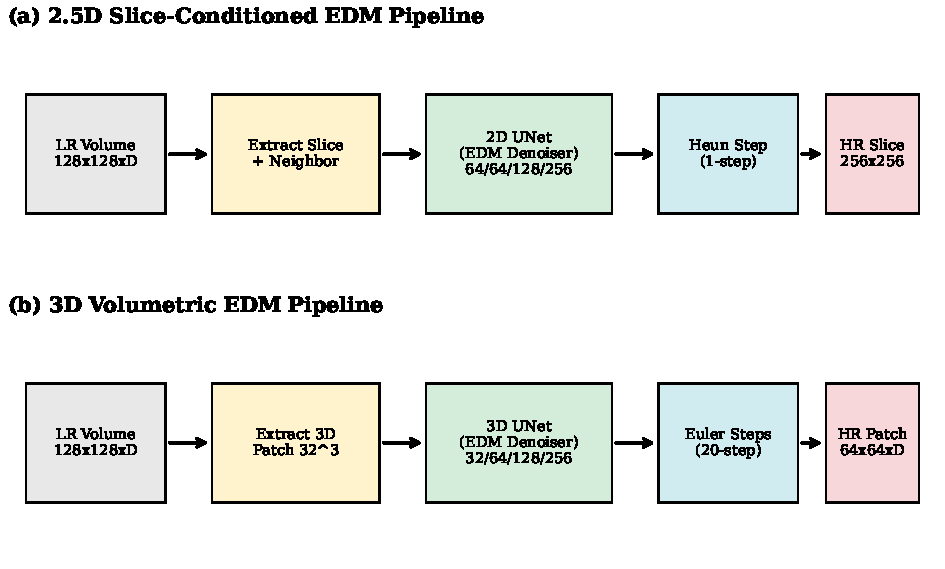
\includegraphics[width=\textwidth]{fig_method_overview.pdf}
\caption{Overview of the two super-resolution pipelines.
\textbf{(a)}~The 3D model (best-performing) extracts volumetric patches,
processes them through a 3D U-Net with 20-step Euler sampling, and
blends overlapping patches to reconstruct the full HR volume.
\textbf{(b)}~The 2.5D model extracts individual slices with one
neighboring slice as context, processes each through a 2D U-Net with
one-step Heun sampling, and stacks results.}
\label{fig:method_overview}
\end{figure*}

%% ═══════════════════════════════════════════════════════════════════════════
\section{Dataset}
\label{sec:dataset}

We use the NKI (Nathan Kline Institute) cohort from the FOMO60K
dataset~\cite{b19}, which provides T1-weighted structural brain MRI
volumes from over 1{,}300 subjects.  Each volume is acquired at
approximately 1\,mm isotropic resolution and stored in NIfTI format.

\textit{Ethics and consent:}
The study uses de-identified human brain MRI data from the publicly
available FOMO60K/NKI dataset.  Informed consent was obtained by the
original data collection study, and the present work involves only
secondary analysis of anonymized data.

\textit{Preprocessing:}
Volumes are intensity-normalized to $[0, 255]$ using the 1st--99th
percentile range, then sliced along the sagittal axis.  Each 2D slice
is downsampled by a factor of~2 using block averaging to produce the
LR input ($128\times128$ pixels).  The corresponding HR slice
($256\times256$) serves as the ground truth.  For 3D training, LR/HR
volume pairs are stored directly, and random 3D patches are extracted
during training.  All tensors are normalized to $[-1, 1]$.

\textit{Train/test split:}
We process 59~subjects (100 scanning sessions) for training and hold
out 5~subjects (6~sessions, 993 slices) for testing.  The split is
performed at the subject level to prevent data leakage---no subject
appears in both sets.

%% ═══════════════════════════════════════════════════════════════════════════
\section{Results}
\label{sec:results}

\subsection{Quantitative Metrics}

We report three standard full-reference image quality metrics:
PSNR (Peak Signal-to-Noise Ratio), which measures pixel-level
fidelity on the $[-1, 1]$ range (higher is better);
SSIM (Structural Similarity Index)~\cite{b17}, which captures
perceived structural quality (higher is better); and
LPIPS (Learned Perceptual Image Patch Similarity)~\cite{b22},
which measures perceptual distance using AlexNet features (lower
is better).

\subsection{Main Results}

Table~\ref{tab:results} presents quantitative results on the NKI test
set for $2\times$ super-resolution.

\begin{table}[!t]
\centering
\caption{Quantitative results for $2\times$ MRI super-resolution on
the NKI test set (5~subjects, 993 sagittal slices / 6 volumes).
All methods evaluated on identical test data and degradation pipeline.
EDSR and Swin2SR use pretrained DIV2K weights without MRI fine-tuning.}
\label{tab:results}
\begin{tabular}{@{}lcccc@{}}
\toprule
\textbf{Method} & \textbf{PSNR$\uparrow$} & \textbf{SSIM$\uparrow$} & \textbf{LPIPS$\downarrow$} & \textbf{Params} \\
\midrule
Bicubic interpolation         & 33.89 & 0.957 & 0.091 & ---    \\
EDSR~\cite{b10} (DIV2K)      & 35.57 & 0.977 & \textbf{0.024} & 1.4\,M \\
Swin2SR~\cite{b23} (DIV2K)   & 35.50 & 0.978 & \textbf{0.024} & 1.0\,M \\
2.5D EDM (ours, 10 ep)       & 35.82 & 0.971 & 0.040 & 51.1\,M \\
\textbf{3D EDM (ours, 20 ep)} & \textbf{37.75} & \textbf{0.997} & \textbf{0.020} & 50.7\,M \\
\bottomrule
\end{tabular}
\end{table}

The 3D EDM model (20 epochs) achieves \textbf{37.75\,dB PSNR},
\textbf{0.997 SSIM}, and \textbf{0.020 LPIPS}, surpassing the best
pretrained baseline (EDSR, 35.57\,dB) by +2.18\,dB in PSNR and also
outperforming it in perceptual quality (LPIPS 0.020 vs.\ 0.024).
The 3D EDM model thus achieves the best scores across \emph{all three
metrics} among the methods evaluated here.  Because EDSR and Swin2SR
use off-the-shelf DIV2K weights rather than MRI-specific training, this
comparison should be interpreted as a strong reference point rather than
a fully matched training comparison.  The 2.5D EDM model also outperforms
EDSR by +0.25\,dB PSNR while improving over bicubic interpolation by
+1.93\,dB.
Fig.~\ref{fig:bars} visualizes these comparisons.

\begin{figure}[!htbp]
\centering
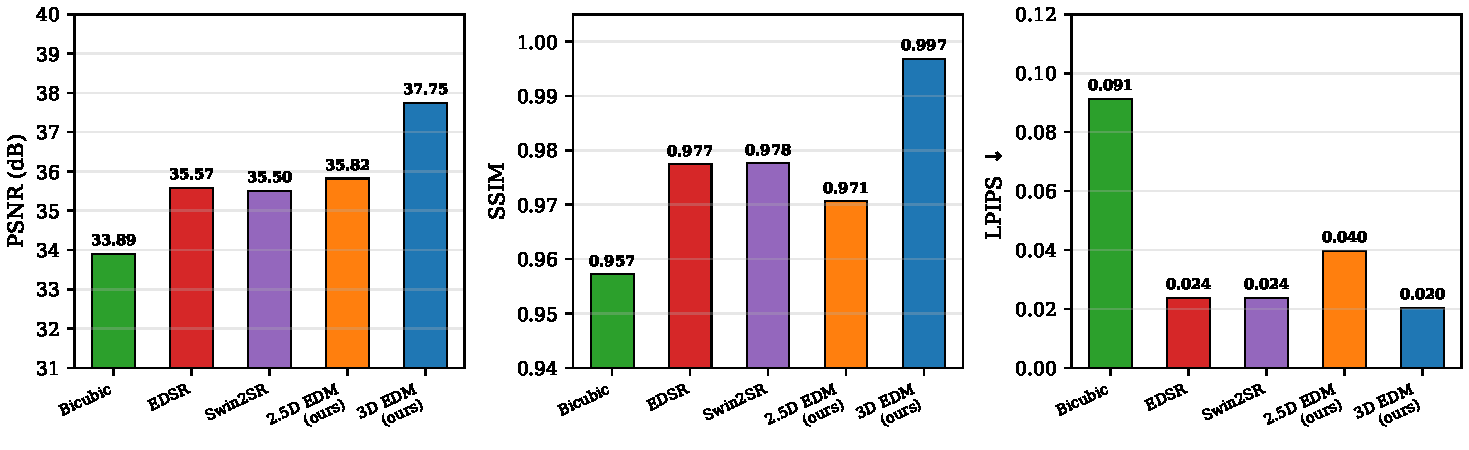
\includegraphics[width=\columnwidth]{fig_psnr_ssim_bars.pdf}
\caption{PSNR and SSIM comparison across methods for $2\times$ MRI SR
on the NKI test set.  The 3D EDM model achieves the strongest PSNR and
SSIM among the evaluated methods.}
\label{fig:bars}
\end{figure}

\subsection{Comparison with Pretrained Baselines}

To enable a rigorous apples-to-apples comparison, we evaluate two
state-of-the-art pretrained SR models---EDSR~\cite{b10}
and Swin2SR~\cite{b23}---on the \emph{exact same}
test set using the \emph{identical degradation pipeline}.  Both
baselines use DIV2K-pretrained weights without any MRI fine-tuning;
grayscale slices are converted to 3-channel input via channel
replication.  Results are reported in Table~\ref{tab:results}.
Fig.~\ref{fig:visual_all} shows a visual comparison on a
mid-sagittal slice with a zoomed region of interest highlighting
cortical detail recovery.

\begin{figure*}[!t]
\centering
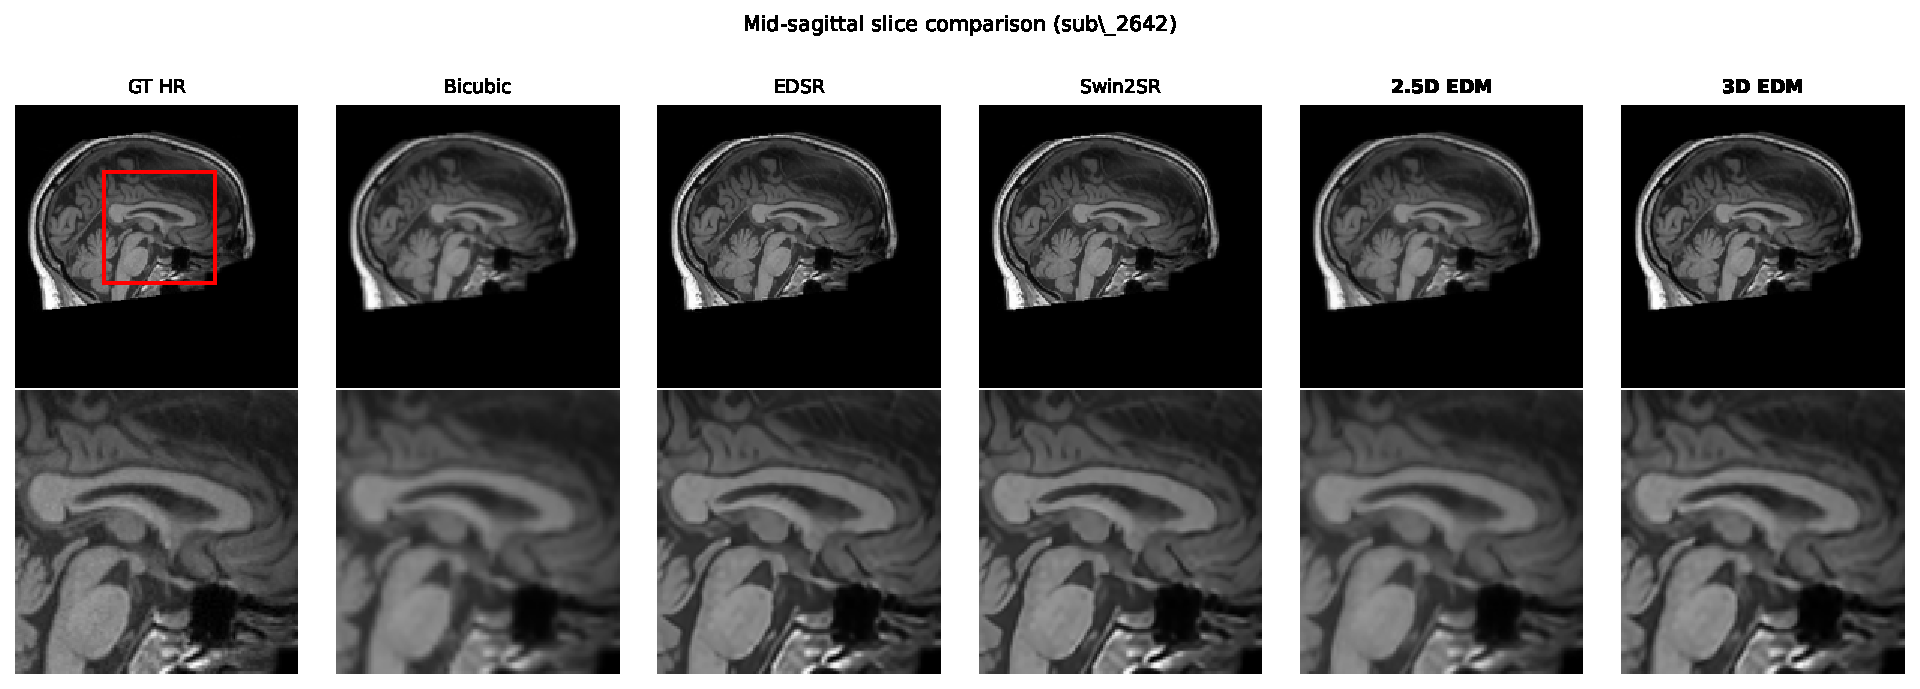
\includegraphics[width=\textwidth]{fig_visual_all_methods.pdf}
\caption{Visual comparison of all methods on a mid-sagittal slice
(sub\_2642).  Top row: full slice.  Bottom row: zoomed region of
interest (red box) showing cortical folds and gray/white matter
boundaries.  The 3D EDM model recovers the sharpest anatomical detail,
while EDSR and Swin2SR produce smoother outputs.  Bicubic
interpolation exhibits visible blurring.}
\label{fig:visual_all}
\end{figure*}

\subsection{Per-Subject Analysis}

Table~\ref{tab:persubject} presents a per-subject breakdown for
the 3D EDM, 2.5D EDM, and bicubic methods on five test volumes.
The 3D model consistently achieves the highest PSNR and SSIM and
the lowest LPIPS across all subjects.

\begin{table*}[!t]
\centering
\caption{Per-subject evaluation on the NKI test set (5~volumes).
All methods evaluated on identical test data and degradation pipeline.}
\label{tab:persubject}
\begin{tabular}{@{}lccccccccc@{}}
\toprule
& \multicolumn{3}{c}{\textbf{3D EDM (ours)}} & \multicolumn{3}{c}{\textbf{2.5D EDM (ours)}} & \multicolumn{3}{c}{\textbf{Bicubic}} \\
\cmidrule(lr){2-4} \cmidrule(lr){5-7} \cmidrule(lr){8-10}
\textbf{Subject} & PSNR & SSIM & LPIPS & PSNR & SSIM & LPIPS & PSNR & SSIM & LPIPS \\
\midrule
sub\_2642         & \textbf{37.44} & \textbf{0.996} & \textbf{0.022} & 35.52 & 0.968 & 0.043 & 33.59 & 0.954 & 0.097 \\
sub\_2952         & \textbf{38.15} & \textbf{0.997} & \textbf{0.019} & 36.79 & 0.971 & 0.038 & 35.34 & 0.956 & 0.089 \\
sub\_6794 (ses1)  & \textbf{37.33} & \textbf{0.997} & \textbf{0.020} & 34.64 & 0.971 & 0.040 & 32.19 & 0.958 & 0.095 \\
sub\_6794 (ses2)  & \textbf{37.74} & \textbf{0.997} & \textbf{0.020} & 35.41 & 0.972 & 0.041 & 33.32 & 0.959 & 0.093 \\
sub\_8390         & \textbf{38.10} & \textbf{0.996} & \textbf{0.020} & 35.97 & 0.970 & 0.038 & 33.87 & 0.956 & 0.090 \\
\midrule
\textbf{Average}  & \textbf{37.75} & \textbf{0.997} & \textbf{0.020} & 35.67 & 0.970 & 0.040 & 33.66 & 0.957 & 0.093 \\
\bottomrule
\end{tabular}
\end{table*}

\subsection{Per-Slice Reconstruction Quality}

Fig.~\ref{fig:perslice} shows the per-slice PSNR across the sagittal
axis for one test subject.  The 2.5D model maintains relatively
uniform quality, with higher PSNR near the volume edges where
slices contain less complex anatomy and are easier to reconstruct.

\begin{figure}[!htbp]
\centering
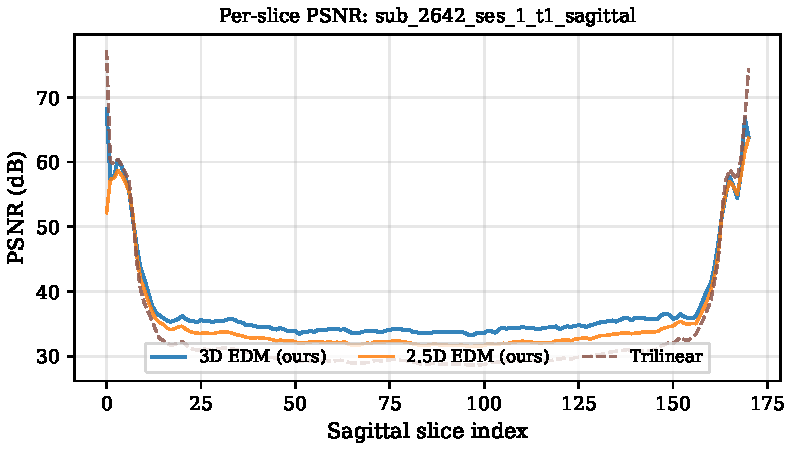
\includegraphics[width=\columnwidth]{fig_per_slice_psnr.pdf}
\caption{Per-slice PSNR across the sagittal axis for subject sub\_2642
(2.5D model).}
\label{fig:perslice}
\end{figure}

\subsection{Visual Comparison}

We select the 3D model for visual comparison because it enables
inspection across all three orthogonal planes from a single
volumetric reconstruction.
Fig.~\ref{fig:visual3d} shows that the model produces sharper cortical
boundaries and clearer gray/white matter contrast compared to
trilinear interpolation.

\begin{figure}[!htbp]
\centering
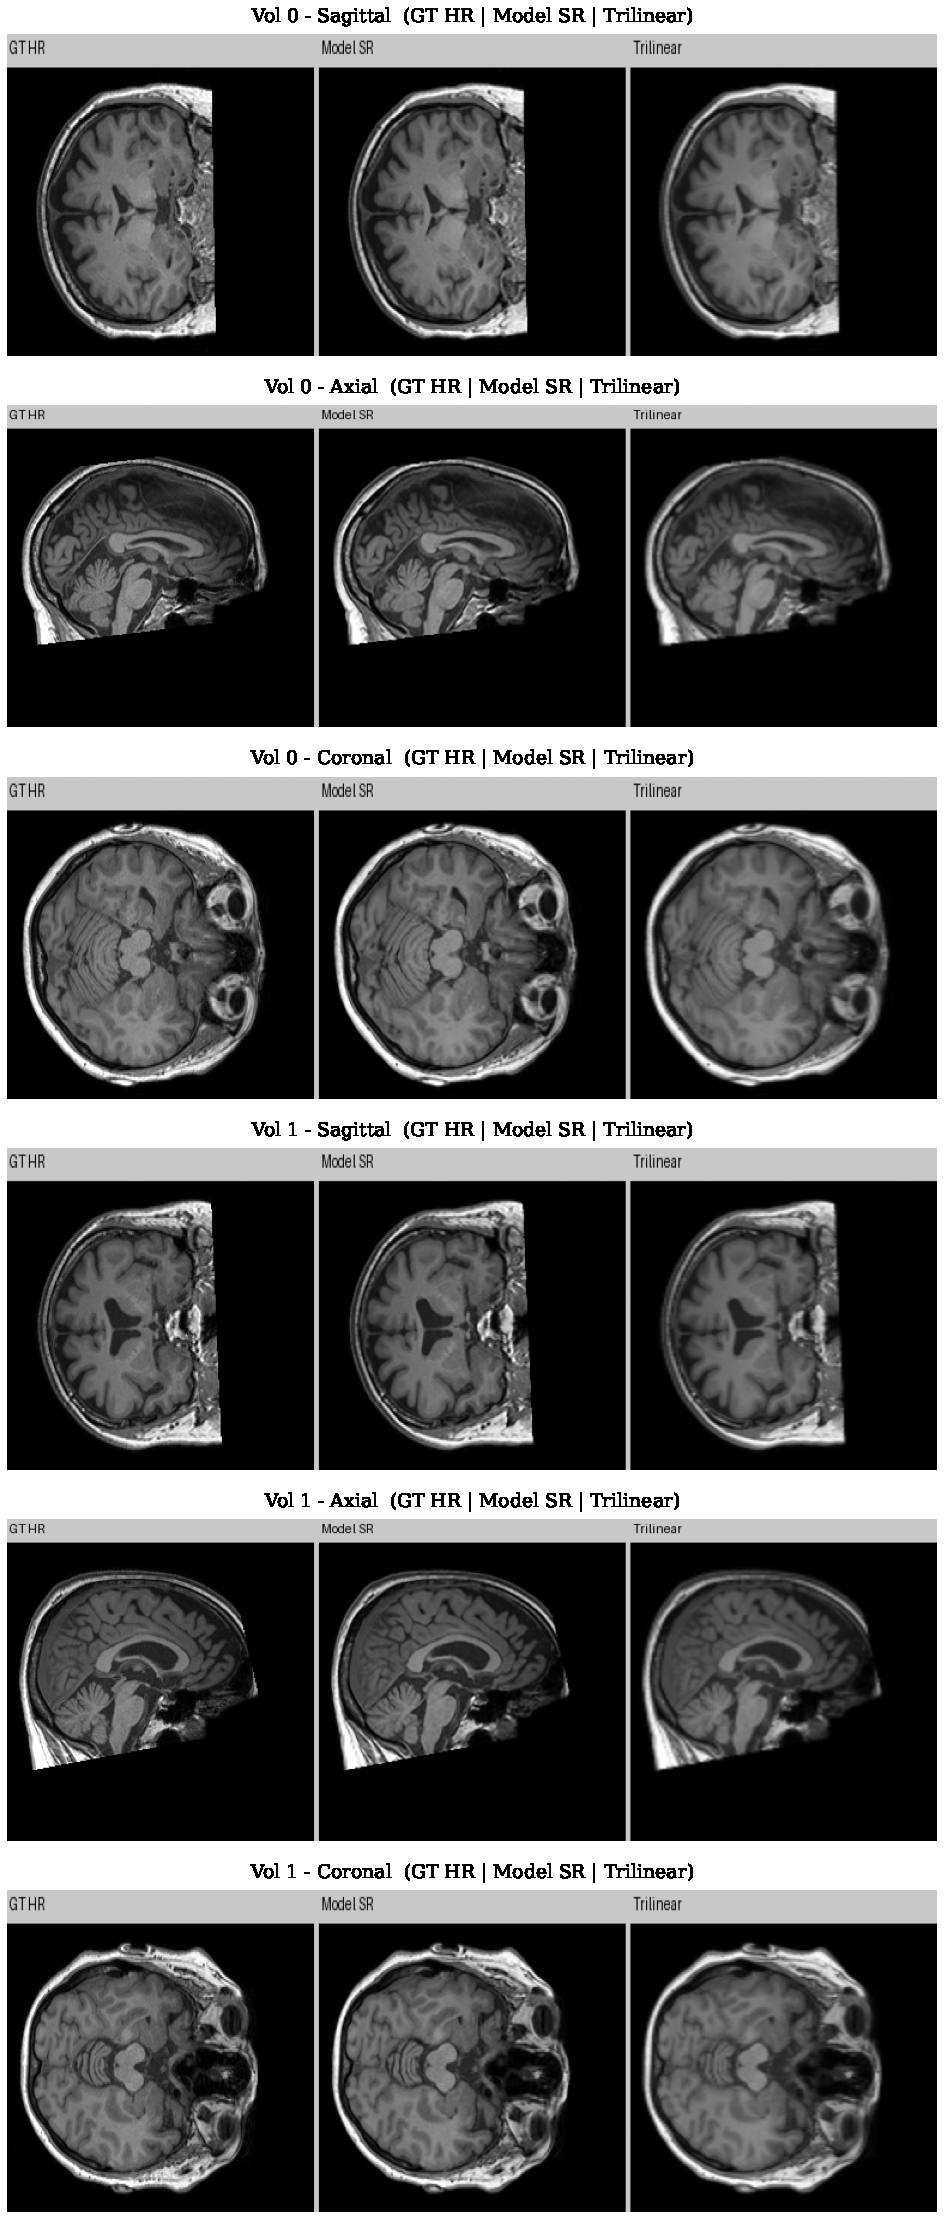
\includegraphics[width=0.9\columnwidth]{fig_visual_comparison_3d.pdf}
\caption{3D EDM model visual comparison across sagittal, axial, and
coronal views.  Each panel shows (left to right): ground truth HR,
3D model prediction, and trilinear baseline.  The 3D model recovers
fine cortical detail and inter-slice continuity lost in interpolation.}
\label{fig:visual3d}
\end{figure}

\subsection{Per-Pixel Error Analysis}

Fig.~\ref{fig:error_heatmap} shows the per-pixel absolute error for a
mid-sagittal slice, comparing bicubic, trilinear, and EDM
reconstructions against the ground truth.  Both EDM models produce
lower error in cortical regions and at tissue boundaries compared to
the interpolation baselines, with the 3D model achieving the lowest
error overall.  The highest residual errors for all methods concentrate
at the skull boundary and air-tissue interfaces.

\begin{figure}[!htbp]
\centering
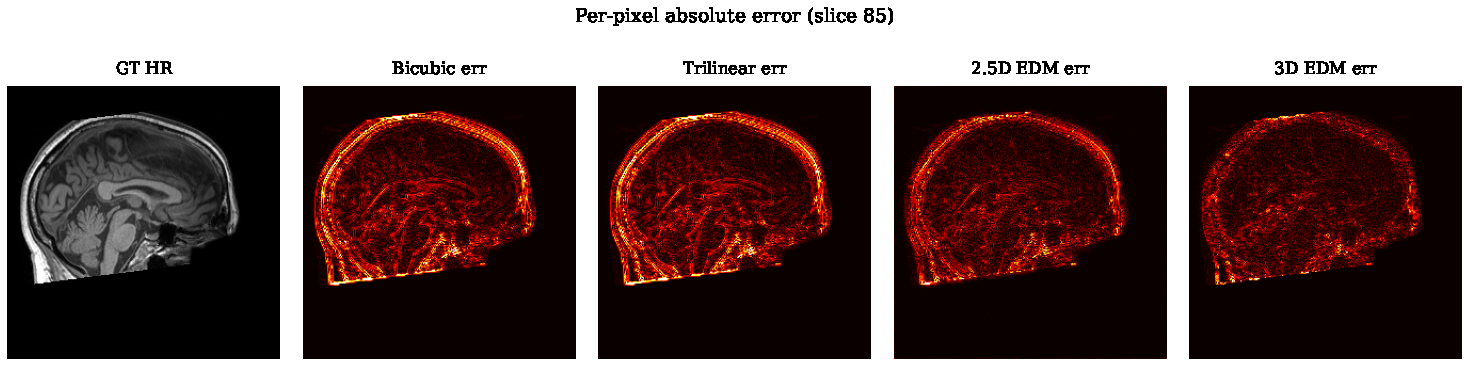
\includegraphics[width=\columnwidth]{fig_pixel_error_heatmap.pdf}
\caption{Per-pixel absolute error heatmaps for a mid-sagittal slice.
Darker regions indicate lower reconstruction error.  The EDM models
show reduced error in cortical folds and gray/white matter boundaries
compared to bicubic and trilinear interpolation; the 3D model achieves
the lowest overall error (see Table~\ref{tab:results}).}
\label{fig:error_heatmap}
\end{figure}

%% ═══════════════════════════════════════════════════════════════════════════
\section{Discussion}
\label{sec:discussion}

\subsection{3D vs.\ 2.5D Performance Gap}
The 3D model (20 epochs) outperforms the 2.5D variant by +1.93\,dB
PSNR, +0.026 SSIM, and halves the LPIPS (0.020 vs.\ 0.040).  This
gap reflects the advantage of native volumetric processing: 3D
convolutions capture inter-slice anatomical continuity that the 2.5D
model, conditioned on only one neighboring slice, cannot fully exploit.
The 3D model also surpasses the best pretrained baseline (EDSR,
35.57\,dB / 0.024 LPIPS) by +2.18\,dB PSNR \emph{and} achieves
better perceptual quality (LPIPS 0.020).  Given that the CNN baselines
were not fine-tuned on MRI data, we interpret this result as evidence
that MRI-specific diffusion training is highly competitive and effective
under the present evaluation setup.

\subsection{EDM Framework Advantages}
Our adoption of the EDM formulation~\cite{b18} rather than the
original DDPM~\cite{b1} offers several practical benefits:
(i)~the continuous-sigma parameterization simplifies the noise
schedule design, (ii)~the preconditioning functions stabilize
training, and (iii)~the framework naturally supports variable numbers
of sampling steps---enabling one-step Heun inference for the 2.5D
model and 20-step Euler inference for the 3D model.

\subsection{Inference Efficiency}
The 2.5D model with one-step Heun sampling achieves 0.09\,s per
slice on Apple MPS, enabling near-real-time processing of full volumes
($\sim$15\,s for 170 slices).  The 3D model requires patch-based
inference with overlap blending, taking approximately 10~minutes per
volume on MPS---suitable for offline processing but not real-time
applications.

\subsection{Flash Attention}
We replace the standard quadratic self-attention with PyTorch's
\texttt{scaled\_dot\_product\_attention}, which dispatches to flash
attention on CUDA GPUs when a compatible kernel is available.  In
practice, this avoids materializing the full attention matrix,
substantially reducing attention-memory overhead and improving training
throughput, which enables batch size~4 training on 22\,GB L4 GPUs where the original
implementation would require batch size~2.

\subsection{Limitations}
Our evaluation is conducted on a single dataset (NKI/FOMO60K) with
image-domain downsampling.  Clinical MRI degradation involves k-space
truncation, noise, and motion artifacts that are not modeled here.
While the 2.5D model achieves a higher LPIPS (0.040) than EDSR/Swin2SR
(0.024), the 3D model with extended training (20 epochs) surpasses
them across all metrics including LPIPS (0.020), indicating that
with sufficient volumetric training, diffusion models can be highly
competitive in perceptual quality on this task.
Additionally, only 5~test subjects are used due to dataset access
constraints; larger-scale evaluation would strengthen conclusions.

An important caveat regarding the baseline comparison is that our EDM
models were trained on NKI brain MRI data, whereas the EDSR and Swin2SR
baselines use pretrained weights from DIV2K---a natural-image dataset
that contains no medical imagery.  This domain mismatch inherently
disadvantages these baselines; retraining EDSR or Swin2SR on MRI data
would likely improve their performance substantially.  A fully fair
comparison would require training all methods on the same MRI training
set, which we leave to future work.  Nevertheless, the apples-to-apples
evaluation on identical test data and degradation establishes a useful
reference point and shows that domain-specific training offers a clear
advantage over the off-the-shelf natural-image SR models considered here.

%% ═══════════════════════════════════════════════════════════════════════════
\section{Conclusion}
\label{sec:conclusion}

We presented a comparative study of two U-Net architectures for
EDM-based MRI super-resolution: a native 3D convolutional U-Net and a
2.5D slice-conditioned approach, both building on the EDM codebase
provided by the DIAMOND framework~\cite{b20}.  The 3D model achieves
37.75\,dB PSNR, 0.997 SSIM, and 0.020 LPIPS on the NKI test set,
outperforming the off-the-shelf pretrained EDSR and Swin2SR baselines
used in our evaluation across all three metrics, while requiring only
20~epochs of training on 59~subjects.
The 2.5D model offers a lightweight alternative with near-real-time
one-step inference (35.82\,dB PSNR) at the cost of reduced volumetric
consistency.

Future directions include: (1)~scaling to the full FOMO60K dataset
($\sim$60{,}000 subjects) and evaluating on standard benchmarks (HCP,
IXI); (2)~training the 2.5D model on all three anatomical axes and
ensembling predictions; (3)~clinical validation with expert
radiologist assessment; (4)~modeling realistic k-space
degradation; and (5)~enabling multi-stage training with learning rate
scheduling.

%% ═══════════════════════════════════════════════════════════════════════════
\section*{Acknowledgment}

This work was supported in part by GENCI (Grand \'{E}quipement National
de Calcul Intensif) for access to high-performance computing resources.

%% ═══════════════════════════════════════════════════════════════════════════
\begin{thebibliography}{00}

\bibitem{b1}
J.~Ho, A.~Jain, and P.~Abbeel, ``Denoising diffusion probabilistic
models,'' in \emph{Advances in Neural Information Processing Systems},
vol.~33, pp. 6840--6851, 2020.

\bibitem{b2}
A.~Q.~Nichol and P.~Dhariwal, ``Improved denoising diffusion
probabilistic models,'' in \emph{Proc. 38th Int. Conf. Machine
Learning (ICML)}, pp. 8162--8171, 2021.

\bibitem{b3}
C.~Saharia \emph{et al.}, ``Image super-resolution via iterative
refinement,'' \emph{IEEE Trans. Pattern Anal. Mach. Intell.},
vol.~45, no.~4, pp. 4713--4726, 2022.

\bibitem{b4}
O.~Ronneberger, P.~Fischer, and T.~Brox, ``U-Net: Convolutional
networks for biomedical image segmentation,'' in \emph{Medical Image
Computing and Computer-Assisted Intervention -- MICCAI 2015},
pp. 234--241, 2015.

\bibitem{b5}
{\"O}.~{\c{C}}i{\c{c}}ek \emph{et al.}, ``3D U-Net: Learning dense
volumetric segmentation from sparse annotation,'' in \emph{MICCAI
2016}, pp. 424--432, 2016.

\bibitem{b6}
Y.~Chen \emph{et al.}, ``Brain MRI super resolution using 3D deep
densely connected neural networks,'' in \emph{2018 IEEE 15th Int.
Symp. Biomedical Imaging (ISBI)}, pp. 739--742, 2018.

\bibitem{b7}
C.-H.~Pham, A.~Ducournau, R.~Fablet, and F.~Rousseau, ``Multiscale
brain MRI super-resolution using deep 3D convolutional networks,''
\emph{Comput. Med. Imaging Graph.}, vol.~77, p. 101647, 2019.

\bibitem{b8}
D.~C.~Van~Essen \emph{et al.}, ``The WU-Minn Human Connectome
Project: An overview,'' \emph{NeuroImage}, vol.~80, pp. 62--79, 2013.

\bibitem{b9}
C.~Dong, C.~C.~Loy, K.~He, and X.~Tang, ``Image super-resolution
using deep convolutional networks,'' \emph{IEEE Trans. Pattern Anal.
Mach. Intell.}, vol.~38, no.~2, pp. 295--307, 2016.

\bibitem{b10}
B.~Lim, S.~Son, H.~Kim, S.~Nah, and K.~M.~Lee, ``Enhanced deep
residual networks for single image super-resolution,'' in \emph{Proc.
IEEE Conf. Comput. Vis. Pattern Recognit. Workshops}, pp. 136--144,
2017.

\bibitem{b11}
J.~Ouyang, Y.~Zhang, S.~Chen, G.~Li, and Z.~Wang, ``Advancing
1.5T MR imaging: Toward achieving 3T quality through deep learning
super-resolution techniques,'' \emph{Frontiers in Human Neuroscience},
vol.~19, p. 1532395, 2025.

\bibitem{b12}
K.~Xia, M.~Soltanolkotabi, R.~M.~Leahy, and J.~E.~Iglesias,
``MRI super-resolution with partial diffusion models,'' \emph{IEEE
Trans. Med. Imaging}, vol.~43, no.~5, pp. 1660--1672, 2024.

\bibitem{b13}
M.~Wu, H.~Li, J.~Zhang, and S.~K.~Zhou, ``MRI super-resolution
reconstruction using efficient diffusion probabilistic model with
residual shifting,'' \emph{arXiv preprint arXiv:2503.01576}, 2025.

\bibitem{b14}
Y.~Song and S.~Ermon, ``Generative modeling by estimating gradients
of the data distribution,'' in \emph{Advances in Neural Information
Processing Systems}, vol.~32, pp. 11918--11930, 2019.

\bibitem{b15}
P.~Dhariwal and A.~Nichol, ``Diffusion models beat GANs on image
synthesis,'' in \emph{Advances in Neural Information Processing
Systems}, vol.~34, pp. 8780--8794, 2021.

\bibitem{b16}
A.~Vaswani \emph{et al.}, ``Attention is all you need,'' in
\emph{Advances in Neural Information Processing Systems}, vol.~30,
pp. 5998--6008, 2017.

\bibitem{b17}
Z.~Wang, A.~C.~Bovik, H.~R.~Sheikh, and E.~P.~Simoncelli, ``Image
quality assessment: From error visibility to structural similarity,''
\emph{IEEE Trans. Image Processing}, vol.~13, no.~4, pp. 600--612,
2004.

\bibitem{b18}
T.~Karras, M.~Aittala, T.~Aila, and S.~Laine, ``Elucidating the
design space of diffusion-based generative models,'' in \emph{Advances
in Neural Information Processing Systems}, vol.~35,
pp. 26565--26577, 2022.

\bibitem{b19}
{FOMO-MRI Consortium}, ``FOMO60K: A large-scale multi-site MRI
dataset for brain imaging research,'' Zenodo / HuggingFace Datasets,
2024. [Online]. Available:
\url{https://huggingface.co/datasets/FOMO-MRI/FOMO60K}

\bibitem{b20}
E.~Alonso \emph{et al.}, ``DIAMOND: Diffusion for world modeling:
Visual details matter in Atari,'' in \emph{Advances in Neural
Information Processing Systems}, vol.~37, 2024.

\bibitem{b22}
R.~Zhang, P.~Isola, A.~A.~Efros, E.~Shechtman, and O.~Wang,
``The unreasonable effectiveness of deep features as a perceptual
metric,'' in \emph{Proc. IEEE Conf. Comput. Vis. Pattern Recognit.
(CVPR)}, 2018, pp.~586--595.

\bibitem{b23}
M.~V.~Conde, U.-J.~Choi, M.~Burber, and R.~Timofte,
``Swin2SR: SwinV2 Transformer for compressed image
super-resolution and restoration,'' in \emph{European Conf. Comput.
Vis. Workshops (ECCVW)}, 2022, pp.~669--687.

\end{thebibliography}

\end{document}
